\documentclass[a4paper,openright,12pt]{book}
\usepackage{graphicx}
\usepackage[sort&compress]{natbib}
\usepackage[spanish]{babel}
\usepackage{epsfig}
\usepackage{rotating}
\usepackage{amsmath}
\usepackage{slashbox}
\usepackage{setspace}
\usepackage{amsfonts}
\usepackage{dcolumn}
\usepackage{multirow}
\usepackage{url}
\usepackage{natbib}
\usepackage{amssymb}
\usepackage{times}
\usepackage{fontspec}
\usepackage{booktabs}
\usepackage{geometry}
\usepackage{cite}
\usepackage{caption}
% \usepackage[utf8]{inputenc}

\setcounter{secnumdepth}{3}
\setmainfont{Times New Roman}
\geometry{left=3cm,right=3cm,top=2.5cm,bottom=2.5cm}

\RequirePackage{ifpdf} % ¿latex o pdflatex?
% Configuración de las imágenes

\usepackage{graphicx}		% Inclusión de imágenes
\DeclareGraphicsExtensions{.pdf}

\graphicspath{ {../imgs/} } % Ruta respecto al fichero tex principal dónde se buscan imágenes

\onehalfspace
\begin{document}

\begin{titlepage}

\begin{center}
\vspace*{-1in}
\begin{figure}[htb]
\begin{center}

\includegraphics[height=2cm]{logo_uz}
\hfill
\includegraphics[height=2cm]{logo_fecem}
\end{center}
\end{figure}
\vspace*{0.15in}
FACULTAD DE CIENCIAS ECONÓMICAS Y EMPRESARIALES \\
\vspace*{0.15in}
DEPARTAMENTO DE ESTRUCTURA ECONÓMICA\\
\vspace*{0.6in}
\begin{large}
TRABAJO\\
\end{large}
\vspace*{0.2in}
\begin{Large}
\textbf{COMERCIO INTERNACIONAL} \\
\end{Large}
\vspace*{0.3in}
\begin{large}
Análisis De La Economía De Chipre \\ 
\end{large}
\vspace*{0.3in}
%\rule{80mm}{0.1mm}\\
%\vspace*{0.1in}
\begin{large}
Autor: \\
Maximiliano Greco \\
\end{large}
\end{center}

\end{titlepage}

\newpage




% -------------- EMPIEZA LA READACCIÓN-----------------------------------------

\chapter{Presentación Del País}
\label{cap1}


\section{Situación Geográfica}


\begin{figure}[htb]
    \centering
    \caption{Situación geográfica de Chipre.}
    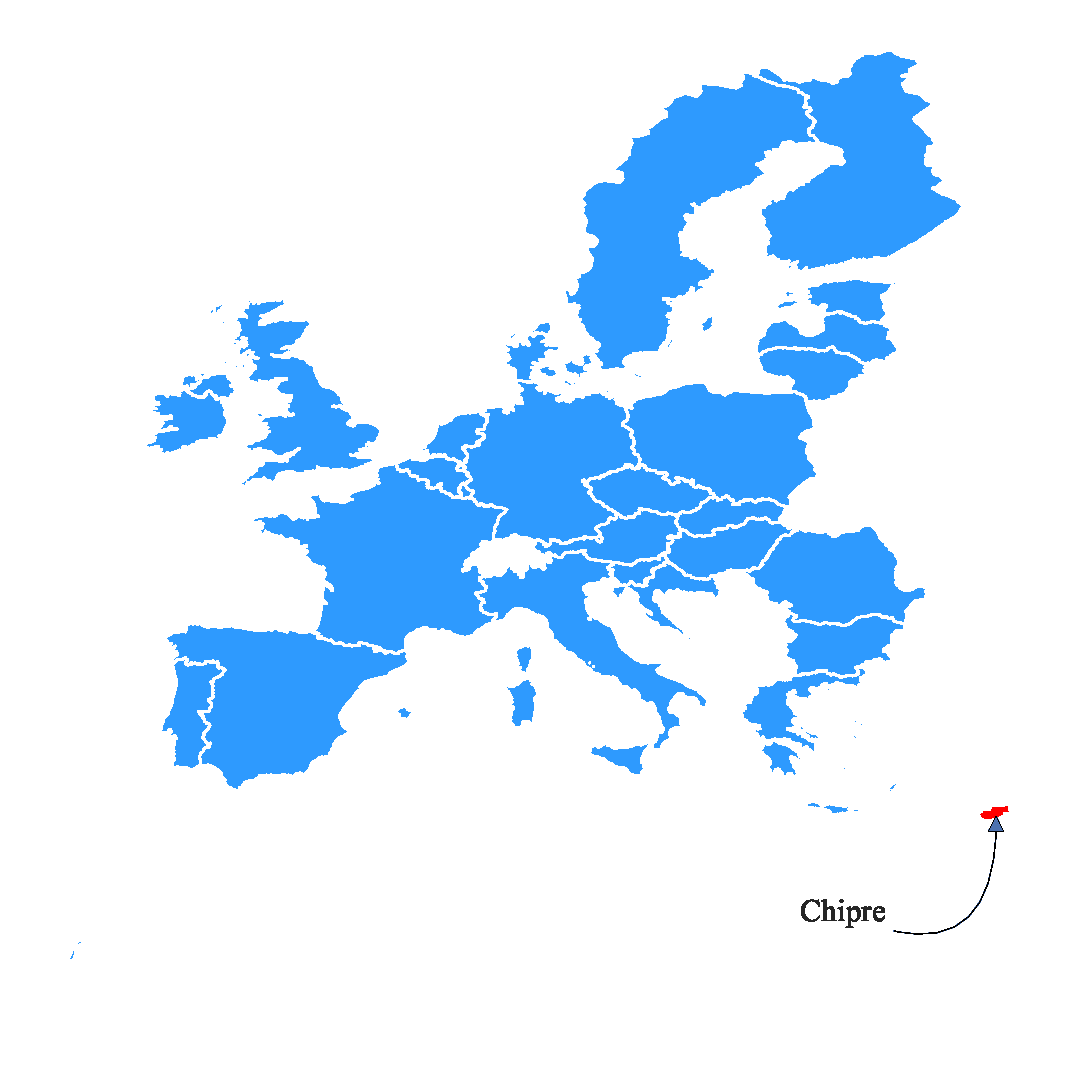
\includegraphics[width=9cm]{mapa}
    \caption*{\textit{Fuente}: Elaboración propia a partir de Shapefile de Eurostat}
    \label{fig1}
\end{figure}

\section{Historia}

Chipre tiene una gran riqueza histórica, ya en la prehistoria disponía de pozos de agua, los más antiguos del mundo[cita], hasta poblados del neolítico[cita]. Chipre ha albergado a diversas cultaras, cómo la Griega y la fenicia (Antigua región orginalmente que en la actualidad iba desde Israel hasta Siria), pasando por Egipcios, persas, el imperio romano, Bizantino (actual Turquía), Árabe, Rep. de Venecia, Turco-Otomana, británica y griega otra vez.

En 1974 se produce un golpe de estado por el gobierno Turco, invadiendo el tercio norte de Chipre, y dando origen a la Rep. Turca del Norte de Chipre (RTNC) formando un estado que sólo reconoce Turquía e ignorado por la comunidad internacional. En 2004 Chipre entra en la Unión Europea.

Chipre se divide en seis distritos:

\begin{enumerate}
    \spacing{0.5}
    \item Nicosia: Se encuentra en la RTNC
    \item Famagusta: Se encuentra en la RTNC
    \item Limassol
    \item Pafos
    \item Lárnaca
    \item Kyrenia: Se encuentra en la RTNC
\end{enumerate}

 Además, en el sur existen dos territorios que son bases militares bajo el mando de Reino Unido.

\begin{enumerate}
    \item Acrotiri
    \item Dhekelia
\end{enumerate}

\begin{figure}[ht]
    \centering
    \caption{Distritos de Chipre}
    \includegraphics[width=9cm]{mapa_distritos.png}
    \caption*{\textit{Fuente}: {ChipreWi33}}
    \label{mapdistrics}
\end{figure}

\section{Recursos Naturales}

Recursos Naturales de Chipre:

\begin{enumerate}
    \spacing{0.5}
    \item cobre
    \item pirita
    \item asbesto
    \item yeso
    \item madera
    \item sal
    \item mármol
    \item tierra de arcilla.
    \item gas natural
    \item petróleo
\end{enumerate}

\*Actualmente se encuentra en fase de exploración y análisis para su futura explotación que se estima a partir 2018-2020.

Fuente: ICEXEspa50

\section{Grupos Económicos}
Por rellenar

\section{Instituciones Internacionales}

Por rellenar

\section{Rasgos Económicos}

Por rellenar

\section{Sectores Releevantes En La Produción Y Comercio Exterior}

Por rellenar

\section{Evolución Macroecnómica Comparada}

Por rellenar

\section{Relación Real de Intercambio}

La relación real de intercambio (RRI) se define cómo $RRI = \frac{P_x}{P_m} = \frac{IVU_x}{IVU_m} 100$ implica, por tanto, que cuando la realación real de intercambio es mayor que 100 entonces el valor de las exportaciones son mayores que el valor de las importaciones (y viceversa), que la RRI sea mayor que 100 implica que para una mismca cantidad de exportaciones el país puede obtener una mayor cantidad de importaciones, lo cual mejora el bienestar, es decir, el comercio internacional reporta beneficios.

\begin{figure}[ht]
    \centering
    \caption{Relación Real de Intercambio de Chipre}
    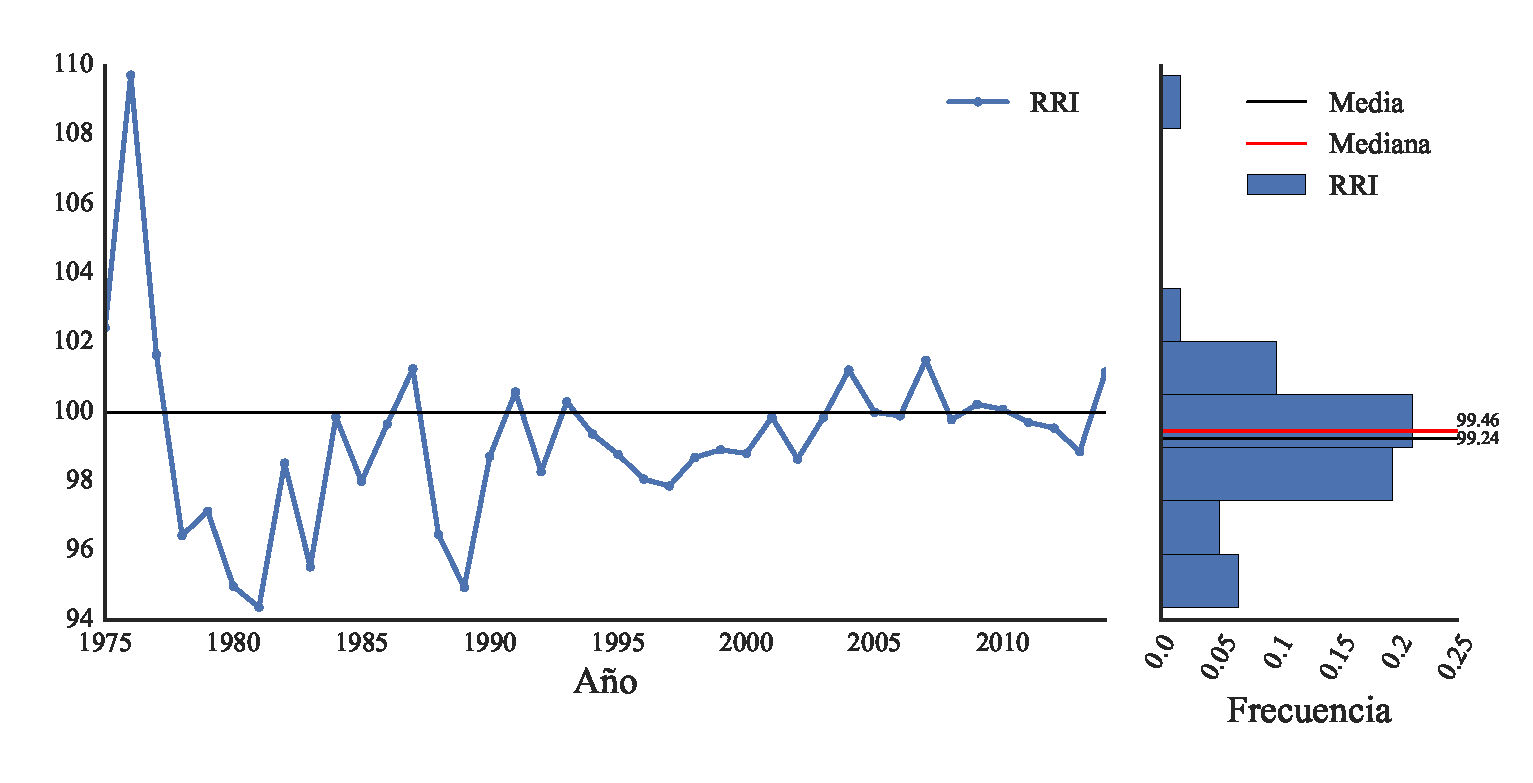
\includegraphics[width=300px]{rri_0}
    \caption*{\textit{Fuente}: Elaboración propia con datos de \textit{World Bank API (WDI)}}
    \label{rri}
\end{figure}

Cómo puede verse en al Figura \ref{rri}, la evolución de la relación real de intercambio de Chipre, gira en torno a un valor por debajo del 100\%, aproximadamente 99.46\% es el porcentaje medio y 99.24\% es el valor de la mediana, como puede constatarse en el histograma de la derecha, mas del 50\% de las observaciones la RRI de chipre se hallan con valores inferiores al 99.24\%, esto estrictamente indica que Chipre pierde bienestar con el comercio internacional, dado que el valor de lo que importa es superior a lo que exporta, lo que implica que para una mismca cantidad de exportaciones cada vez puede importar menos. En el periodo analizado sin duda Chipre ha perdido bienestar con el comercio internacional con más frecuencia que el que ha ganado.


\chapter{Evolución Del Comercio}
\label{cap2}

\begin{sidewaystable}[ht]
    \centering
    \caption{Evolución de los Últimos 10 años del comercio de Chipre}
    \label{}
    \resizebox{\textwidth}{!}{%
    \begin{tabular}{lllllllllllll}
    \toprule
    {} &  \multicolumn{1}{|p{3cm}|}{\centering Importaciones de \\ BBSS (moneda local)} &  \multicolumn{1}{|p{3cm}|}{\centering Exportaciones de \\ BBSS (moneda local)} &  \multicolumn{1}{|p{3cm}|}{\centering Crecimiento nominal \\ de las importaciones (\%)} &  \multicolumn{1}{|p{3cm}|}{\centering Crecimiento nominal \\ de las exportaciones (\%)} &  \multicolumn{1}{|p{3cm}|}{\centering Crecimiento real \\ de las importaciones (\%)} &  \multicolumn{1}{|p{3cm}|}{\centering Crecimiento real \\ de las exportaciones (\%)} & \multicolumn{1}{|p{3cm}|}{\centering Saldo comercial \\ (LCU)} &  \multicolumn{1}{|p{3cm}|}{\centering Saldo Comercial \\ (\% PIB)} &  \multicolumn{1}{|p{3cm}|}{\centering Tasa de \\ Cobertura (\%)} &  \multicolumn{1}{|p{3cm}|}{\centering Tasa de\\ Apertura (\%)} & \multicolumn{1}{|p{3cm}|}{\centering  Penetración\\ de las Importaciones (\%)} &  \multicolumn{1}{|p{3cm}|}{\centering Propensión\\ Exportadora} \\
    Año &                                       &                                       &                                               &                                               &                                            &                                            &                        &                          &                        &                       &                                       &                         \\
    \midrule
    2000 & 7.155.010.000,00                     & 7.412.550.000,00                     & 14,38                                         & 13,81                                         & 9,21                                       & 8,79                                       & 257.540.000,00        & 2,44                     & 103,60                 & 138,27                & 69,62                                 & 70,36                  \\
    2001 & 7.265.740.000,00                     & 7.787.330.000,00                     & 1,55                                          & 5,06                                          & -0,19                                      & 2,18                                       & 521.590.000,00        & 4,60                     & 107,18                 & 132,73                & 67,15                                 & 68,66                  \\
    2002 & 7.273.030.000,00                     & 7.411.900.000,00                     & 0,10                                          & -4,82                                         & -0,36                                      & -4,09                                      & 138.870.000,00        & 1,18                     & 101,91                 & 124,45                & 62,37                                 & 62,81                  \\
    2003 & 7.224.510.000,00                     & 7.419.710.000,00                     & -0,67                                         & 0,11                                          & -0,97                                      & -1,40                                      & 195.200.000,00        & 1,53                     & 102,70                 & 114,81                & 57,52                                 & 58,17                  \\
    2004 & 7.900.090.000,00                     & 7.882.900.000,00                     & 9,35                                          & 6,24                                          & 6,95                                       & 2,49                                       & -17.190.000,00        & -0,13                    & 99,78                  & 114,94                & 57,46                                 & 57,41                  \\

    2005 &                      8.333.840.000,00 &                      8.254.850.000,00 &                                          5,49 &                                          4,72 &                                       1,57 &                                       2,05 &         -78.990.000,00 &                    -0,54 &                  99,05 &                112,92 &                                 56,42 &                   56,19 \\
    2006 &                      9.019.310.000,00 &                      8.549.730.000,00 &                                          8,23 &                                          3,57 &                                       5,70 &                                       1,27 &        -469.580.000,00 &                    -2,97 &                  94,79 &                110,94 &                                 55,31 &                   53,99 \\
    2007 &                     10.159.530.000,00 &                      9.326.470.000,00 &                                         12,64 &                                          9,08 &                                      10,46 &                                       5,28 &        -833.060.000,00 &                    -4,81 &                  91,80 &                112,45 &                                 55,94 &                   53,82 \\
    2008 &                     11.440.420.000,00 &                      9.417.380.000,00 &                                         12,61 &                                          0,97 &                                       7,74 &                                      -1,72 &      -2.023.040.000,00 &                   -10,78 &                  82,32 &                111,13 &                                 55,02 &                   50,18 \\
    2009 &                      9.550.060.000,00 &                      8.721.350.000,00 &                                        -16,52 &                                         -7,39 &                                     -16,05 &                                      -7,28 &        -828.710.000,00 &                    -4,50 &                  91,32 &                 99,18 &                                 49,61 &                   47,34 \\
    2010 &                     10.157.580.000,00 &                      9.095.460.000,00 &                                          6,36 &                                          4,29 &                                       4,52 &                                       2,63 &      -1.062.120.000,00 &                    -5,57 &                  89,54 &                101,00 &                                 50,47 &                   47,71 \\
    2011 &                     10.319.010.000,00 &                      9.653.110.000,00 &                                          1,59 &                                          6,13 &                                      -0,62 &                                       4,21 &        -665.900.000,00 &                    -3,42 &                  93,55 &                102,49 &                                 51,20 &                   49,54 \\
    2012 &                     10.028.060.000,00 &                      9.653.370.000,00 &                                         -2,82 &                                          0,00 &                                      -4,60 &                                      -1,66 &        -374.690.000,00 &                    -1,93 &                  96,26 &                101,39 &                                 50,68 &                   49,73 \\
    2013 &                      8.759.650.000,00 &                      9.209.850.000,00 &                                        -12,65 &                                         -4,59 &                                     -13,61 &                                      -4,99 &         450.200.000,00 &                     2,48 &                 105,14 &                 99,18 &                                 49,58 &                   50,83 \\
    2014 &                      9.220.300.000,00 &                      9.704.100.000,00 &                                          5,26 &                                          5,37 &                                       8,07 &                                       5,72 &         483.800.000,00 &                     2,76 &                 105,25 &                108,10 &                                 54,17 &                   55,43 \\

    \bottomrule
\end{tabular}}
\caption*{\textit{Fuente}: Elaboración propia con datos de World Bank API.}
\end{sidewaystable}

\section{Nominal}


\begin{figure}[htb]
    \caption{Evolución de las exportaciones (por uno) y su frecuencia.}
    \centering
    \includegraphics[width=300px]{ev_nominal.pdf}
    \caption*{\textit{Fuente}: Elaboración propia con datos de World Bank API.}
    \label{ev_nominal}
\end{figure}

Tanto las importaciones cómo las exportaciones se han visto afectadas nominalmente en 2008 por la crisis económica, se puede ver en la caída de éstas en el gráfico. En los últimos 10 años, el crecimiento de ambas variables ha estado girando en torno al 2\% siendo las exportaciones ligeramente superior a las importaciones haciendo que el crecimiento del saldo exterior sea positivo pero muy discreto de magnitud de un 0.2\%. Es interesante que ver que sólo el 20\% de los años el crecimiento de las exportaciones presentó valores negativos (30\% para las importaciones) esto se debe principalmente, cómo veremos en el siguiente gráfico, a la inflación.


\section{Real}


\begin{table}[]
\centering
\caption{Evolución de las importaciones de Chipre.}
\label{tab2}
\begin{tabular}{@{}lll@{}}
\toprule
date & \multicolumn{1}{l}{\begin{tabular}[c]{@{}l@{}}Importaciones de \\ bienes y servicios \\ (constante LCU)\end{tabular}} & \multicolumn{1}{l}{\begin{tabular}[c]{@{}l@{}}Importaciones de \\ bienes y servicios \\ (corriente LCU)\end{tabular}} \\ \midrule
1980 & 2.676.118.100,00                                                                                                      & 819.274.400,00                                                                                                        \\
1981 & 2.743.072.900,00                                                                                                      & 947.761.300,00                                                                                                        \\
1982 & 3.094.066.300,00                                                                                                      & 1.124.943.200,00                                                                                                      \\
1983 & 3.264.572.800,00                                                                                                      & 1.242.495.000,00                                                                                                      \\
1984 & 3.798.964.600,00                                                                                                      & 1.533.298.900,00                                                                                                      \\
1985 & 3.626.378.900,00                                                                                                      & 1.489.900.500,00                                                                                                      \\
1986 & 3.229.223.700,00                                                                                                      & 1.324.507.800,00                                                                                                      \\
1987 & 3.688.343.200,00                                                                                                      & 1.529.027.400,00                                                                                                      \\
1988 & 4.176.573.800,00                                                                                                      & 1.824.615.500,00                                                                                                      \\
1989 & 5.015.381.800,00                                                                                                      & 2.308.833.100,00                                                                                                      \\
1990 & 5.302.331.700,00                                                                                                      & 2.493.703.900,00                                                                                                      \\
1991 & 5.407.130.200,00                                                                                                      & 2.609.205.300,00                                                                                                      \\
1992 & 6.403.969.100,00                                                                                                      & 3.214.904.500,00                                                                                                      \\
1993 & 5.226.227.600,00                                                                                                      & 2.681.479.100,00                                                                                                      \\
1994 & 5.597.598.500,00                                                                                                      & 2.999.449.800,00                                                                                                      \\
1995 & 6.531.110.000,00                                                                                                      & 5.192.630.000,00                                                                                                      \\
1996 & 6.842.650.000,00                                                                                                      & 5.636.820.000,00                                                                                                      \\
1997 & 6.926.900.000,00                                                                                                      & 5.909.750.000,00                                                                                                      \\
1998 & 6.963.940.000,00                                                                                                      & 5.998.680.000,00                                                                                                      \\
1999 & 7.133.060.000,00                                                                                                      & 6.255.730.000,00                                                                                                      \\
2000 & 7.790.250.000,00                                                                                                      & 7.155.010.000,00                                                                                                      \\
2001 & 7.775.370.000,00                                                                                                      & 7.265.740.000,00                                                                                                      \\
2002 & 7.747.590.000,00                                                                                                      & 7.273.030.000,00                                                                                                      \\
2003 & 7.672.140.000,00                                                                                                      & 7.224.510.000,00                                                                                                      \\
2004 & 8.205.030.000,00                                                                                                      & 7.900.090.000,00                                                                                                      \\
2005 & 8.333.830.000,00                                                                                                      & 8.333.840.000,00                                                                                                      \\
2006 & 8.809.070.000,00                                                                                                      & 9.019.310.000,00                                                                                                      \\
2007 & 9.730.760.000,00                                                                                                      & 10.159.530.000,00                                                                                                     \\ \bottomrule
\end{tabular}
\caption*{\textit{Fuente}: Elaboración propia con datos de \textit{WDI}}
\end{table}


\begin{figure}[ht]
    \caption{Evolución de las importaciones (por uno) y su frecuencia.}
    \centering
    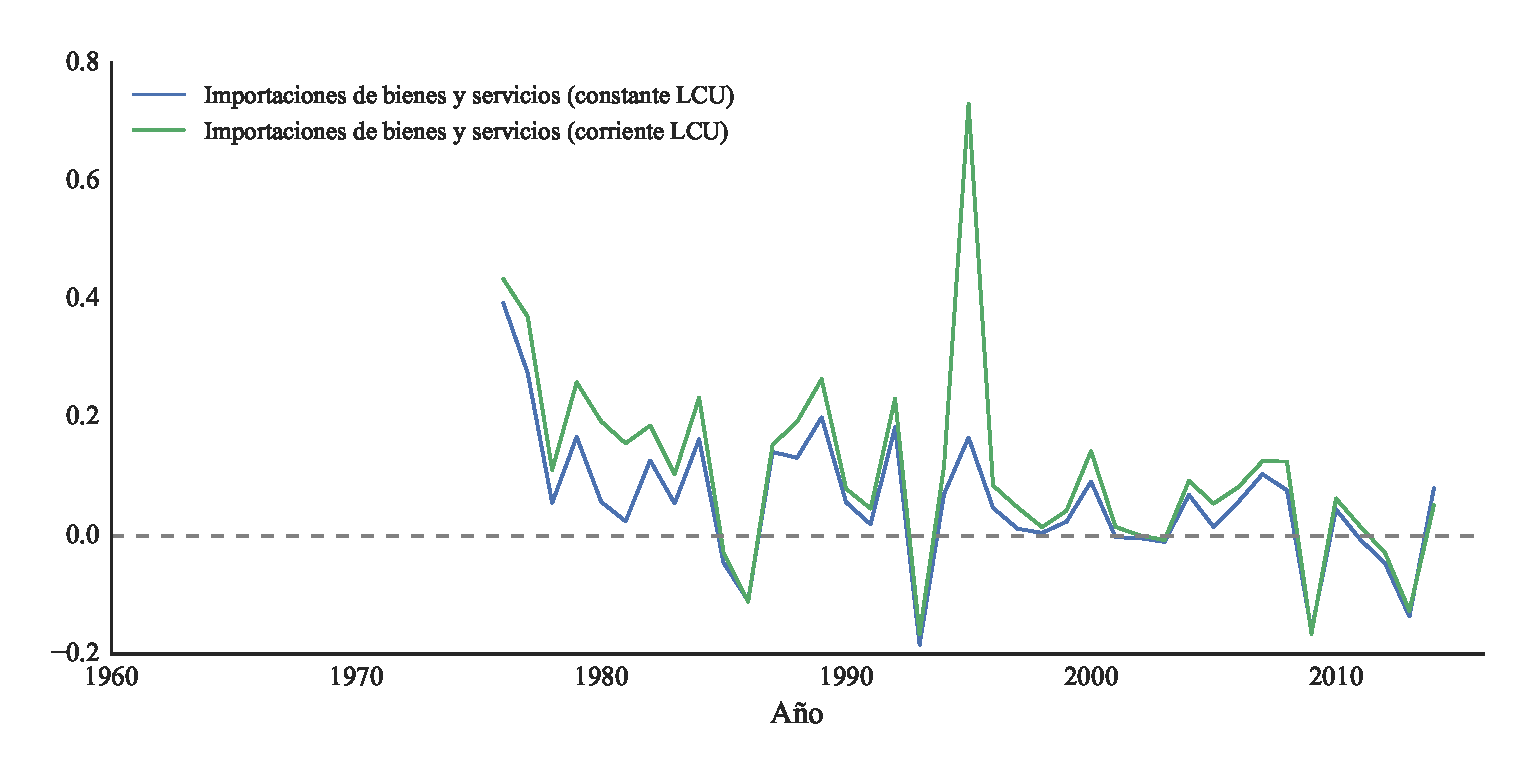
\includegraphics[width=300px]{ev_m}
    \label{ev_m}
\end{figure}


\chapter{Distribución Geográfica De M y X}
\label{cap3}

En este apartado se analizan los principales socios comerciales que tiene Chipre, tanto proveedores cómo clientes, y se identifican las posibles causas explicativas para que sean esos paises y no otros los que comercian con Chipre. En primer luga se presentan los pesos de las importaciones por paises con el fin de identificar los pricipales proveedores de Chipre. En segundo lugar, se obtienen y muestran los pricipales países a los que Chipre exporta, con lo que se identifica los principales clientes de Chipre. De esta forma tenemos caracterizados los clientes y proveedores.

En la base de datos \textit{PC-TAS}, obtenemos los principales socios comerciales, exportando los datos de allí, y ordenando los pesos tenemos dos tablas, que se resúmen en las siguientes figuras:

\begin{figure}[ht]
    \centering
    \caption{Peso de las importaciones para los principales socios comerciales}
    \includegraphics[width=350px]{pie_mgeo.pdf}
    \caption*{\textit{Fuente}: Elaboración propia con datos de \textit{PC-TAS}}
    \label{pie_mgeo}
\end{figure}

\begin{figure}[ht]
    \centering
    \caption{Peso de las importaciones de los principales socios comerciales}
    \includegraphics[width=350px]{bar_mgeo.pdf}
    \caption*{\textit{Fuente}: Elaboración propia con datos de \textit{PC-TAS}}
    \label{bar_mgeo}
\end{figure}

Los principales orígenes de las importaciones de Chipre son países de la propia unión europea como muestra la Figura REF, pero destaca sobre el resto las importaciones procedentes de Grecia con casi el doble de peso sobre el esto, diferencia que se ha mantenido desde 2007 hasta 2011.
Estas relaciones se pueden explicar con el pasado geopolítico de Chipre, que pasó a estar a menos de UK, luego Grecia y con una cultura... continuar

\begin{figure}[ht]
    \centering
    \caption{Peso de las exportaciones de los principales socios comerciales}
    \includegraphics[width=350px]{pie_xgeo.pdf}
    \caption*{\textit{Fuente}: Elaboración propia con datos de \textit{PC-TAS}}
    \label{pie_xgeo}
\end{figure}

\begin{figure}[tbh]
    \centering
    \caption{Peso de las exportaciones de los principales socios comerciales}
    \includegraphics[width=350px]{bar_xgeo.pdf}
    \caption*{\textit{Fuente}: Elaboración propia con datos de \textit{PC-TAS}}
    \label{bar_xgeo}
\end{figure}


Las exportaciones de Chipre tienen como principales destinos, Grecia, Para Buques, Reino Unido, Alemania y Rumanía, que juntas tiene un peso de 58.69\% en 2007 y 56.79\% en 2011. Cómo puede verse en la Figura REF, las exportaciones de 2007 hacia Grecia y Para Buques aumentaron en 2011, mientras que el resto disminuyeron.
Los destinos concuerdan con la historia Chipriota, fué una colonia y de Reino Unido, y formó parte de Grecia, esta dependencia del pasado ha hecho que se mantenga hasta hoy en día nexos comerciales fuertes.

\subsubsection{El modelo de Gravedad}

Según el modelo de gravedad en su forma más general, definida de la siguiente manera:

\begin{equation}
T_{ij} = A \cdot Y_i^a \cdot \frac{Y_j^b}{D_{ij}^c}
\end{equation}

dónde, $T_i_j$ es el valor del comercio entre el país _i_ y el país _j_, $Y_i^a$ es el PIB del país _i_, $Y_j^b$ es el PIB del país j y $D_i_j$ es la distancia entre los dos países

La pregunta que cabe hacerse es si el comercio entre Chipre y estos países siguen el comportamiento previsto por el modelo de gravedad, y para eso hay que analizar la distancia entre los paises, el PIB. A priori, sin datos, Reino Unido tiene una distancia menor y un PIB mayor que Grecia, sin embargo, el peso de las exportaciones es menor que el de Grecia, esto a grandes rasgos sugiere que no se cumpmle el modelo de Gravedad, para un analisis riguroso necesitamos, los datos y hacer un análisis econométrico.

\chapter{Competitividad Precio O Coste}
\label{cap4}

\chapter{Competitividad Estructural}
\label{cap5}

\chapter{Especialización comercial}
\label{cap6}

ESPECIALIZACIÓN COMERCIAL

\begin{figure}[ht]
    \centering
    \caption{Distribución de sectores por SCR vs IDEP, IESP}
    \includegraphics[width=400px]{cuadrantes2.pdf}
    \caption*{\textit{Fuente}: Elaboración propia con datos de \textit{PC-TAS}}
    \label{sec_scr_idep_iesp}
\end{figure}


\chapter{Comercio Intraindustrial}

Este capítulo se centra en el análisis del comercio intraindustrial de Chipre, para lo cual se analizan un conjunto de indicadores a partir de los datos obtenidos de la BBDD, Pc-Tas sobre importación y exportación de Chipre. Los datos están desagregado por sectores y por destino/origen. Una descripción de los indicadores usados se encuentra en el \ref{anexo}, entre ellos se usarán: el peso de las importaciones, el índice de especialización, el índice de dependencia, saldo comercial relativo y el índice de Grubel y Lloyd AÑADIR CITA, cada uno en su contexto.

Para anlizar el comercio, se han seleccionado los sectores mas importantes según el peso sobre el PIB y dentro de ese grupo, se han elegido aquellos sectore que tienen un indice de especialización mayor que ### y un índice de dependecia mayor que ###.


\begin{figure}[ht]
    \centering
    \caption{Indicadores de especialización comercial por cuadrantes para cada sector}
    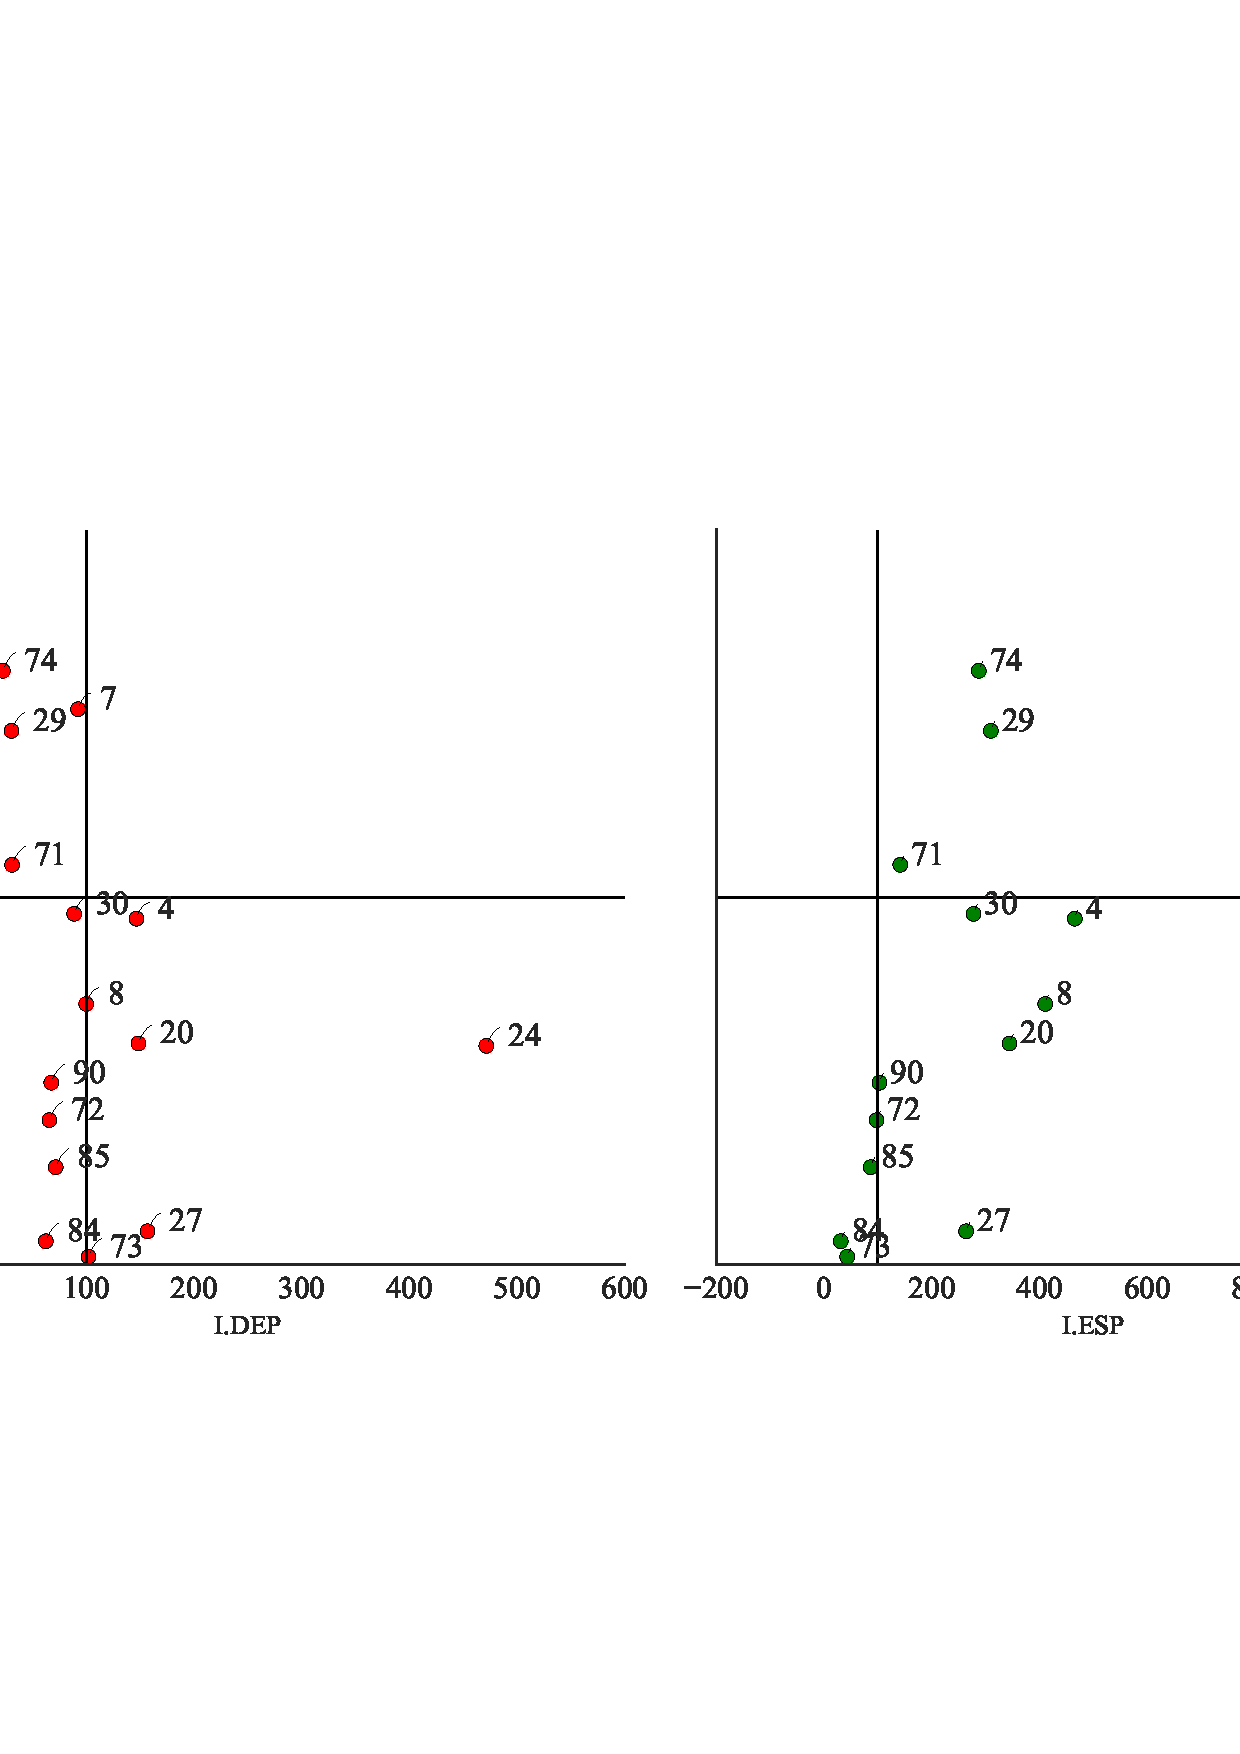
\includegraphics[width=450px]{cuadrantes.pdf}
    \caption*{\textit{Fuente}: Elaboración propia con datos de \textit{PC-TAS}}
    \label{esp_c}
\end{figure}

\begin{table}[ht]
    \centering
    \caption{Descipción de Cuadrantes}
    \label{desc_cuadrantes}
    \begin{tabular}{@{}lcc@{}}
    \toprule
                       & I.DEP \textgreater 100 & I.ESP \textgreater 100 \\ \midrule
    SCR \textgreater 0 & Cuadrante 1      & Cuadrante 2      \\
    SCR \textless 0    & Cuadrante 3  & Cuadrante 4     \\ \bottomrule
    \end{tabular}
\end{table}


\begin{table}[ht]
    \centering
    \caption{Cuadrante 2}
    \label{tab_c2}
    \resizebox{\textwidth}{!}{%
    \begin{tabular}{@{}lllllll@{}}
    \toprule
    & idep                                                                                                          & iesp  & scr      & irx   & irm  & igl  &       \\ \midrule
    Plantas vivas y productos de la floricultura                                                                  & 92,44 & 1.061,90 & 40,98 & 4,40 & 0,41 & 59,02 \\
    Combustibles minerales, aceites minerales y productos de su destilación; materias bituminosas;ceras minerales & 30,67 & 309,79   & 36,25 & 8,74 & 0,92 & 63,75 \\
    Sombreros, demás tocados y sus partes.                                                                        & 31,18 & 141,60   & 7,07  & 2,71 & 0,53 & 92,93 \\
    Manufacturas de piedra, yeso fraguable, cemento, amianto (asbesto), mica o materias análogas                  & 22,60 & 287,38   & 49,33 & 2,86 & 0,22 & 50,67 \\ \bottomrule
    \end{tabular}
    }
    \caption*{\textit{Fuente}: Elaboración propia con datos de \textit{PC-TAS}}
\end{table}

\begin{figure}[ht]
    \centering
    \caption{Indicadores de especialización comerciale por cuadrantes para cada sector}
    \includegraphics[width=250px]{esp_c2.pdf}
    \caption*{\textit{Fuente}: Elaboración propia con datos de \textit{PC-TAS}}
    \label{esp_c2}
\end{figure}

\begin{table}[ht]
    \centering
    \caption{Cuadrante 3}
    \label{tab_c3}
    \resizebox{\textwidth}{!}{%
    \begin{tabular}{@{}lllllll@{}}
    \toprule
    & idep                                                                                                          & iesp   & scr      & irx     & irm   & igl   &       \\ \midrule
    Pescados y crustáceos, moluscos y demás invertebrados acuáticos                                               & 146,76 & 465,79   & -4,65   & 4,19  & 1,03  & 95,35 \\
    Hortalizas, plantas, raíces y tubérculos alimenticios                                                         & 100,05 & 410,83   & -23,23  & 1,94  & 0,70  & 76,77 \\
    Café, té, yerba mate y especias                                                                               & 486,01 & 0,00     & -100,00 & 0,00  & 1,93  & 0,00  \\
    Cacao y sus preparaciones                                                                                     & 148,51 & 344,54   & -31,82  & 1,53  & 0,67  & 68,18 \\
    Preparaciones de hortalizas, frutas u otros frutos o demás partes de plantas                                  & 261,89 & 58,27    & -85,23  & 0,66  & 1,87  & 14,77 \\
    Bebidas, líquidos alcohólicos y vinagre                                                                       & 471,69 & 1.009,57 & -32,35  & 3,53  & 1,55  & 67,65 \\
    Sal; azufre; tierras y piedras; yesos, cales y cementos                                                       & 157,01 & 263,79   & -72,73  & 17,79 & 25,28 & 27,27 \\
    Abonos                                                                                                        & 254,63 & 29,80    & -92,11  & 0,31  & 1,67  & 7,89  \\
    Madera, carbón vegetal y manufacturas de madera                                                               & 125,75 & 19,91    & -91,52  & 0,36  & 1,81  & 8,48  \\
    Guata, fieltro y tela sin tejer, hilados especiales; cordeles, cuerdas y cordajes; artículos de cordelería    & 124,37 & 36,79    & -92,45  & 0,31  & 1,75  & 7,55  \\
    Alfombras y demás revestimientos para el suelo, de materia textil                                             & 152,07 & 24,69    & -94,97  & 0,26  & 2,22  & 5,03  \\
    Plumas y plumón preparados y artículos de plumas o plumón; flores artificiales; manufacturas de cabello       & 102,22 & 42,95    & -78,29  & 0,97  & 1,79  & 21,71 \\
    Reactores nucleares, calderas, máquinas, aparatos y artefactos mecánicos; partes de estas máquinas o aparatos & 184,26 & 47,49    & -87,96  & 0,66  & 2,33  & 12,04 \\ \bottomrule
    \end{tabular}
    }
    \caption*{\textit{Fuente}: Elaboración propia con datos de \textit{PC-TAS}}
\end{table}

\begin{figure}[ht]
    \centering
    \caption{Indicadores de especialización comerciale por cuadrantes para cada sector}
    \includegraphics[width=250px]{esp_c3.pdf}
    \caption*{\textit{Fuente}: Elaboración propia con datos de \textit{PC-TAS}}
    \label{esp_c3}
\end{figure}

\begin{table}[ht]
    \centering
    \caption{Cuadrante 4}
    \label{tab_c4}
    \resizebox{\textwidth}{!}{%
    \begin{tabular}{@{}lllllll@{}}
    \toprule
    & idep                                                                                                                                                          & iesp   & scr      & irx    & irm   & igl   &       \\ \midrule
    Pescados y crustáceos, moluscos y demás invertebrados acuáticos                                                                                               & 146,76 & 465,79   & -4,65  & 4,19  & 1,03  & 95,35 \\
    Hortalizas, plantas, raíces y tubérculos alimenticios                                                                                                         & 100,05 & 410,83   & -23,23 & 1,94  & 0,70  & 76,77 \\
    Cacao y sus preparaciones                                                                                                                                     & 148,51 & 344,54   & -31,82 & 1,53  & 0,67  & 68,18 \\
    Bebidas, líquidos alcohólicos y vinagre                                                                                                                       & 471,69 & 1.009,57 & -32,35 & 3,53  & 1,55  & 67,65 \\
    Sal; azufre; tierras y piedras; yesos, cales y cementos                                                                                                       & 157,01 & 263,79   & -72,73 & 17,79 & 25,28 & 27,27 \\
    Productos químicos inorgánicos; compuestos inorgánicos u orgánicos de metal precioso, de elementos radiactivos, de metales de las tierras raras o de isótopos & 88,85  & 277,71   & -3,60  & 14,37 & 3,46  & 96,40 \\
    Estaño y sus manufacturas                                                                                                                                     & 67,61  & 102,81   & -40,37 & 3,32  & 1,75  & 59,63 \\ \bottomrule
    \end{tabular}
    }
    \caption*{\textit{Fuente}: Elaboración propia con datos de \textit{PC-TAS}}
\end{table}

\begin{figure}[ht]
    \centering
    \caption{Indicadores de especialización comerciale por cuadrantes para cada sector}
    \includegraphics[width=250px]{esp_c4.pdf}
    \caption*{\textit{Fuente}: Elaboración propia con datos de \textit{PC-TAS}}
    \label{esp_c4}
\end{figure}

\chapter{Política Comercial}

\chapter{Resumen y Conclusiones}

% ––––––––––––––––––––––––––––––– ANEXO –––––––––––––––––––––––––––––––––

\chapter{Anexo}

En el Capítulo \ref{cap1} se han usado los siguientes indicadores:

\begin{enumerate}

    \item BALANZA COMERCIAL

    $$X - M$$
    \item TASA DE COBERTURA

    $$\frac{X}{M}100$$
    \item PENETRACIÓN DE LAS IMPORTACIONES

    $$\frac{M}{\text{PIB} + M - X} 100$$
    \item GRADO DE APERTURA

    $$\frac{X+M}{\text{PIB}} 100$$
    \item PROPENSIÓN EXPORTADORA

    $$\frac{X}{\text{PIB}} 100$$

\end{enumerate}

En el Capítulo \ref{cap3}:

\begin{enumerate}
    \item COMPETITIVIDAD PRECIO O COSTE
    \begin{enumerate}
        \item Indices de tipo de cambio efectivo real
        \item Tipo de cambio oficial
        \item Tasa de inflación
    \end{enumerate}

\item ESPECIALIZACIÓN COMERCIAL

\item  INDICE DE DEPENDENCIA

Para todo país $h$ y el sector $i$

$$IDep^h_i = \frac{\frac{M^h_i}{\sum_i M^h_i}}{\frac{\sum_h M^h_i}{\sum_h \sum_i M^h_i}} 100$$

\item  INDICE DE ESPECIALIZACIÓN

$$IEsp^h_i = \frac{\frac{X^h_i}{\sum_i X^h_i}}{\frac{\sum_h X^h_i}{\sum_h \sum_i X^h_i}} 100$$

\item  SALDO COMERCIAL RELATIVO

$$SCR_i = \frac{X_i - M_i}{X_i + M_i} 100$$

\item IMPORTANCIA RELATIVA DEL SECTOR EN LAS IMPORTACIONES Y EXPORTACIONES.

$$IRX_i = \frac{X_i}{\sum_i X_i}$$

$$IRM_i = \frac{M_i}{\sum_i M_i}$$

\item COMERCIO INTRAINDUSTRIAL

$$IGL_i = \frac{X_i + M_i - |X_i - M_i|}{X_i + M_i}100$$

$$IGL_{agg} = \frac{\sum_i(X_i + M_i) - \sum_i |X_i - M_i|}{\sum_i (X_i + M_i)}100$$

\end{enumerate}

En el Capítulo \ref{cap6}:

\begin{enumerate}

    \item INDICE DE DEPENDENCIA

    Para todo país $h$ y el sector $i$

    \begin{equation}
    IDep^h_i = \frac{\frac{M^h_i}{\sum_i M^h_i}}{\frac{\sum_h M^h_i}{\sum_h \sum_i M^h_i}} 100
    \end{equation}

    \item INDICE DE ESPECIALIZACIÓN

    \begin{equation}
    IEsp^h_i = \frac{\frac{X^h_i}{\sum_i X^h_i}}{\frac{\sum_h X^h_i}{\sum_h \sum_i X^h_i}} 100
    \end{equation}

    \item SALDO COMERCIAL RELATIVO

    \begin{equation}
    SCR_i = \frac{X_i - M_i}{X_i + M_i} 100
    \end{equation}

    \item IMPORTANCIA RELATIVA DEL SECTOR EN LAS IMPORTACIONES Y EXPORTACIONES.

    \begin{equation}
    IRX_i = \frac{X_i}{\sum_i X_i}
    \end{equation}

    \begin{equation}
    IRM_i = \frac{M_i}{\sum_i M_i}
    \end{equation}

\end{enumerate}

\subsection{Capítulos Arancelarios}

% Please add the following required packages to your document preamble:
% \usepackage{booktabs}
% \usepackage{graphicx}
\begin{table}[]
\centering
\caption{Capítulos arancelarios}
\label{arm}
\resizebox{\textwidth}{!}{%
\begin{tabular}{@{}ll@{}}
\toprule
cod & descripción                                                                                                                                                                                                                                                                                    \\ \midrule
1   & Animales vivos                                                                                                                                                                                                                                                                                 \\
2   & Carne y Despojos Comestibles                                                                                                                                                                                                                                                                   \\
3   & Pescados y crustáceos, moluscos y demás invertebrados acuáticos                                                                                                                                                                                                                                \\
4   & Leche y productos lácteos; huevos de ave; miel natural; productos comestibles de origen animal, no expresados ni comprendidos en otra parte                                                                                                                                                    \\
5   & Los demás productos de origen animal, no expresados ni comprendidos en otra parte                                                                                                                                                                                                              \\
6   & Plantas vivas y productos de la floricultura                                                                                                                                                                                                                                                   \\
7   & Hortalizas, plantas, raíces y tubérculos alimenticios                                                                                                                                                                                                                                          \\
8   & Frutas y frutos comestibles; cortezas de agrios (cítricos), melones o sandías                                                                                                                                                                                                                  \\
9   & Café, té, yerba mate y especias                                                                                                                                                                                                                                                                \\
10  & Cereales .                                                                                                                                                                                                                                                                                     \\
11  & Productos de la molinería; malta; almidón y fécula; inulina; gluten de trigo                                                                                                                                                                                                                   \\
12  & Semillas y frutos oleaginosos; semillas y frutos diversos; plantas industriales o medicinales; paja y forraje                                                                                                                                                                                  \\
13  & Gomas, resinas y demás jugos y extractos vegetales                                                                                                                                                                                                                                             \\
14  & Materias trenzables y demás productos de origen vegetal, no expresados ni comprendidos en otra parte                                                                                                                                                                                           \\
15  & Grasas y aceites animales o vegetales; productos de su desdoblamiento; grasas alimenticias elaboradas;ceras de origen animal o vegetal                                                                                                                                                         \\
16  & Preparaciones de carne, pescado o de crustáceos, moluscos o demás invertebrados acuáticos                                                                                                                                                                                                      \\
17  & Azúcares y artículos de confitería                                                                                                                                                                                                                                                             \\
18  & Cacao y sus preparaciones                                                                                                                                                                                                                                                                      \\
19  & Preparaciones a base de cereales, harina, almidón, fécula o leche; productos de pastelería                                                                                                                                                                                                     \\
20  & Preparaciones de hortalizas, frutas u otros frutos o demás partes de plantas                                                                                                                                                                                                                   \\
21  & Preparaciones alimenticias diversas                                                                                                                                                                                                                                                            \\
22  & Bebidas, líquidos alcohólicos y vinagre                                                                                                                                                                                                                                                        \\
23  & Residuos y desperdicios de las industrias alimentarias; alimentos preparados para animales                                                                                                                                                                                                     \\
24  & Tabaco y sucedáneos del tabaco, elaborados                                                                                                                                                                                                                                                     \\
25  & Sal; azufre; tierras y piedras; yesos, cales y cementos                                                                                                                                                                                                                                        \\
26  & Minerales metalíferos, escorias y cenizas                                                                                                                                                                                                                                                      \\
27  & Combustibles minerales, aceites minerales y productos de su destilación; materias bituminosas;ceras minerales                                                                                                                                                                                  \\
28  & Productos químicos inorgánicos; compuestos inorgánicos u orgánicos de metal precioso, de elementos radiactivos, de metales de las tierras raras o de isótopos                                                                                                                                  \\
29  & Productos químicos orgánicos                                                                                                                                                                                                                                                                   \\
30  & Productos farmacéuticos                                                                                                                                                                                                                                                                        \\
31  & Abonos                                                                                                                                                                                                                                                                                         \\
32  & Extractos curtientes o tintóreos; taninos y sus derivados; pigmentos y demás materias colorantes; pinturas y barnices; mástiques; tintas                                                                                                                                                       \\
33  & Aceites esenciales y resinoides; preparaciones de perfumería, tocador o cosmética                                                                                                                                                                                                              \\
34  & Jabón, agentes de superficie orgánicos, preparaciones para lavar, preparaciones lubricantes, ceras artificiales, ceras preparadas, productos de limpieza, velas y artículos similares, pastas para modelar, “ceras para odontología” y preparaciones para odontología a base de yeso fraguable \\
35  & Materias albuminóideas; productos a base de almidón o de fécula modificados;colas; enzimas                                                                                                                                                                                                     \\
36  & Pólvora y explosivos; artículos de pirotecnia; fósforos (cerillas); aleaciones pirofóricas; materias inflamables                                                                                                                                                                               \\
37  & Productos fotográficos o cinematográficos                                                                                                                                                                                                                                                      \\
38  & Productos diversos de las industrias químicas                                                                                                                                                                                                                                                  \\
39  & Plástico y sus manufacturas                                                                                                                                                                                                                                                                    \\
40  & Caucho sus manufacturas                                                                                                                                                                                                                                                                        \\
41  & Pieles (excepto la peletería) y cueros                                                                                                                                                                                                                                                         \\
42  & Manufacturas de cuero; artículos de talabartería o guarnicionería; artículos de viaje, bolsos de mano (carteras) y continentes similares; manufacturas de tripa                                                                                                                                \\
43  & Peletería y confecciones de peletería; peletería facticia o artificial                                                                                                                                                                                                                         \\
44  & Madera, carbón vegetal y manufacturas de madera                                                                                                                                                                                                                                                \\
45  & Corcho y sus manufacturas                                                                                                                                                                                                                                                                      \\
46  & Manufacturas de espartería o cestería                                                                                                                                                                                                                                                          \\
47  & Pasta de Madera o de las demás materias fibrosas celulósicas; papel o cartón para reciclar (desperdicios y desechos)                                                                                                                                                                           \\
48  & Papel y cartón; manufacturas de pasta de celulosa, de papel o cartón                                                                                                                                                                                                                           \\
49  & Productos editoriales de la prensa y de las demás industrias gráficas; textos manuscritos o mecanografiados y planos                                                                                                                                                                           \\
50  & Seda                                                                                                                                                                                                                                                                                           \\
51  & Lana y pelo fino u ordinario; hilados y tejidos de crin                                                                                                                                                                                                                                        \\
52  & Algodón                                                                                                                                                                                                                                                                                        \\
53  & Las demás fibras textiles vegetales; hilados de papel y tejidos de hilados de papel                                                                                                                                                                                                            \\
54  & Filamentos sintéticos o artificiales                                                                                                                                                                                                                                                           \\
55  & Fibras sintéticas o artificiales discontinuas                                                                                                                                                                                                                                                  \\
56  & Guata, fieltro y tela sin tejer, hilados especiales; cordeles, cuerdas y cordajes; artículos de cordelería                                                                                                                                                                                     \\
57  & Alfombras y demás revestimientos para el suelo, de materia textil                                                                                                                                                                                                                              \\
58  & Tejidos especiales; superficies textiles con mechón insertado; encajes; tapicería; pasamanería; bordados                                                                                                                                                                                       \\
59  & Telas impregnadas, recubiertas, revestidas o estratificadas; artículos técnicos de materia textil                                                                                                                                                                                              \\
60  & Tejidos de punto                                                                                                                                                                                                                                                                               \\
61  & Prendas y complementos (accesorios), de vestir, de punto                                                                                                                                                                                                                                       \\
62  & Prendas y complementos (accesorios), de vestir, excepto los de punto                                                                                                                                                                                                                           \\
63  & Los demás artículos textiles confeccionados; juegos prendería y trapos                                                                                                                                                                                                                         \\
64  & Calzado, polainas y artículos análogos; partes de estos artículos                                                                                                                                                                                                                              \\
65  & Sombreros, demás tocados y sus partes.                                                                                                                                                                                                                                                         \\
66  & Paraguas, sombrillas, quitasoles, bastones, bastones asiento, látigos, fustas y sus partes                                                                                                                                                                                                     \\
67  & Plumas y plumón preparados y artículos de plumas o plumón; flores artificiales; manufacturas de cabello                                                                                                                                                                                        \\
68  & Manufacturas de piedra, yeso fraguable, cemento, amianto (asbesto), mica o materias análogas                                                                                                                                                                                                   \\
69  & Productos cerámicos                                                                                                                                                                                                                                                                            \\
70  & Vidrio y sus manufacturas                                                                                                                                                                                                                                                                      \\
71  & Perlas finas (naturales)* o cultivadas, piedras preciosas o semipreciosas, metales preciosos, electromecánicos) de señalización para vías de comunicación                                                                                                                                      \\
72  & Fundición, hierro y acero .                                                                                                                                                                                                                                                                    \\
73  & Manufacturas de fundición, hierro o acero                                                                                                                                                                                                                                                      \\
74  & Cobre y sus manufacturas                                                                                                                                                                                                                                                                       \\
75  & Níquel y sus manufacturas                                                                                                                                                                                                                                                                      \\
76  & Aluminio y sus manufacturas                                                                                                                                                                                                                                                                    \\
77  & (Reservado para una futura utilización en el Sistema Armonizado)                                                                                                                                                                                                                               \\
78  & Plomo y sus manufacturas                                                                                                                                                                                                                                                                       \\
79  & Cinc y sus manufacturas                                                                                                                                                                                                                                                                        \\
80  & Estaño y sus manufacturas                                                                                                                                                                                                                                                                      \\
81  & Los demás metales comunes; cermets; manufacturas de estas materias                                                                                                                                                                                                                             \\
82  & Herramientas y útiles, artículos de cuchillería y cubiertos de mesa, de metal común; partes de estos artículos, de metal común                                                                                                                                                                 \\
83  & Manufacturas diversas de metal común                                                                                                                                                                                                                                                           \\
84  & Reactores nucleares, calderas, máquinas, aparatos y artefactos mecánicos; partes de estas máquinas o aparatos                                                                                                                                                                                  \\
85  & Máquinas, aparatos y material eléctrico, y sus partes; aparatos de grabación o reproducción de sonido, aparatos de grabación o reproducción de imagen y sonido en televisión, y las partes y accesorios de estos aparatos.                                                                     \\
86  & Vehículos y material para vías férreas o similares, y sus partes; aparatos mecánicos (incluso electromecánicos) de señalización para vías de comunicación                                                                                                                                      \\
87  & Vehículos automóviles, tractores, velocípedos y demás vehículos terrestres; sus partes y accesorios                                                                                                                                                                                            \\
88  & Aeronaves, vehículos espaciales y sus partes                                                                                                                                                                                                                                                   \\
89  & Barcos y demás artefactos flotantes                                                                                                                                                                                                                                                            \\
90  & Instrumentos y aparatos de óptica. fotografía o cinematografía, de medida, control o precisión; instrumentos y aparatos medicoquirúrgicos; partes y accesorios de estos instrumentos o aparatos                                                                                                \\
91  & Aparatos de relojería y sus partes                                                                                                                                                                                                                                                             \\
92  & Instrumentos musicales; sus partes y accesorios                                                                                                                                                                                                                                                \\
93  & Armas, municiones, y sus partes y accesorios                                                                                                                                                                                                                                                   \\
94  & Muebles; mobiliario medicoquirúrgico; artículos de cama y similares; aparatos de alumbrado no expresados ni comprendidos en otra parte; anuncios, letreros y placas indicadoras luminosos y artículos similares; construcciones prefabricadas                                                  \\
95  & Juguetes, juegos y artículos para recreo o deporte; sus partes y accesorios                                                                                                                                                                                                                    \\
96  & Manufacturas diversas de metal común                                                                                                                                                                                                                                                           \\
97  & Objetos de arte o colección y antigüedades                                                                                                                                                                                                                                                     \\
98  & (Reservado para usos particulares por las Partes Contratantes)                                                                                                                                                                                                                                 \\
99  & (Reservado para usos particulares por las Partes Contratantes)                                                                                                                                                                                                                                 \\
0   & Tratamientos arancelarios especiales                                                                                                                                                                                                                                                           \\ \bottomrule
\end{tabular}%
}
\end{table}


\cleardoublepage
\addcontentsline{toc}{chapter}{Bibliografía}
\bibliographystyle{apalike}
\bibliography{biblio.bib} % yyyy.bib es el fichero donde está salvada la bibliografía.


\end{document}
